%% ------------------------------------------------------------------------- %%n
\chapter{Aprendizado Ativo}
\label{cap:aprendizado_ativo}

Nesse capítulo serão apresentados os fundamentos de aprendizado ativo. É importante citar que muitos dos trabalhos clássicos citados foram descobertos, principalmente, pela revisão da literatura de [\cite{settles2012active, settles2014active}]. Alguns outros trabalhos são também muito importantes nessa discussão, como os de [\cite{olsson2009literature}], focada em Linguagem Natural, o de [\cite{aggarwal2014active}] e de [\cite{wang2011active}]. A própria revisão de literatura de [\cite{zhu2006semi}] também explica alguns conceitos fundamentais e a relação com o aprendizado semi-supervisionado.

O Aprendizado Ativo recebeu bastante atenção até meados de 2010. Em 2011, por exemplo, tivemos um workshop de aprendizado ativo no ICML (International Conference of Machine Learning). Após essa fase tivemos um período com poucos trabalhos e apenas em 2016 tivemos um outro workshop dentro do I-KNOW (International Conference on Knowledge Technologies and Data-driven Business). Em 2017 e 2018 foi criado o workshop international de aprendizado interativo, que engloba aprendizado ativo e áreas correlacionadas como aprendizado semi-supervisionado.

É importante notar que é difícil colocar o aprendizado ativo em alguma categoria específica do aprendizado computacional, normalmente dividido em aprendizado supervisionado, não supervisionado  e por reforço. Primeiro porque o aprendizado computacional, por si só, tem um objetivo muito amplo e é complicado encaixar diferentes frameworks em apenas essas três categorias [\cite{abu2012learning}]. Em segunda lugar porque a própria literatura não possui um consenso a respeito do aprendizado ativo. Por exemplo, [\cite{settles2012active, zhu2006semi}] colocam-o como um framework relacionado ao semi-supervisionado, mas não dentro dele. Outros trabalhos, entretanto, colocam como um subgrupo do aprendizado semi-supervisionado. E há ainda outros, como a pesquisa de Olson [\cite{olsson2009literature}], focada em Linguagem Natural, que o classifica como sendo da estrutura de supervisionado. 

\section{Definição do Aprendizado Ativo}
\label{sec:definicao}

O aprendizado supervisionado tradicional pressupõe que existe um grande conjunto de amostras pré-rotuladas para serem utilizadas no treinamento. Dessa forma, é induzido uma hipótese sobre esses dados, resultando em um classificador [\cite{settles2014active}]. Em contraste a esse aprendizado, também chamado de aprendizado passivo, o aprendizado ativo  é uma técnica que nasce quando não temos dados anotados suficiente e quando o custo envolvido para essa rotulação é proibitivo. A ideia central do aprendizado ativo é que o algoritmo selecione as amostras mais importantes para o treinamento. 


A origem desse paradigma se iniciou com trabalhos que visavam exclusivamente a seleção de amostras mais informativas [\cite{angluin1988queries, baum1992query, atlas1990training}]. Em 1994 o trabalho de [\cite{cohn1994improving}] explicitou o termo e o framework de Aprendizado Ativo e, a partir daquele momento, houveram melhorias e avanços nessa área de pesquisa. 


Na prática, a diferença fundamental é que o primeiro requer que o especialista rotule um grande volume de amostras indiferentemente de eles serem relevantes ou não no processo de aprendizado. Já no aprendizado ativo o algoritmo determina quais amostras podem ser mais úteis para o aprendizado e solicita apenas a rotulação das amostras selecionadas. 

\cite{persello2012active} definem, em seu trabalho, esse tipo de paradigma através de uma quíntupla (G,Q,S,T,U):
\newline
\newline
~~~ G - um classificador inicial 
\newline
~~~ Q - uma política de seleção de amostras a ser enviada ao oráculo (query)
\newline 
~~~ S - um oráculo
\newline 
~~~ T - um conjunto de amostras rotuladas
\newline 
~~~ U - um conjunto de amostras não rotuladas


A figura ~\ref{fig:framework_AL_classico_etapa_inicial} mostra o processo inicial, onde temos uma grande base de amostras não rotuladas U. Note que três amostras são selecionadas e rotuladas corretamente, gerando o conjunto inicial T. Após isso, essas amostras servem como base de treinamento e geramos um classificador. A partir disso é possível iniciar o processo interativo do aprendizado ativo.


\begin{figure}
  \centering
  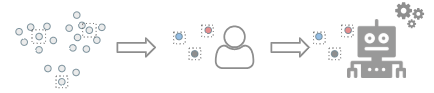
\includegraphics[width=.9\textwidth]{figures/Framework_processo_inicial.png}
  \caption{Etapa Inicial do Framework de Aprendizado Ativo}
  \label{fig:framework_AL_classico_etapa_inicial}
\end{figure}


No processo interativo já temos um classificador e um conjunto de amostras pré-rotuladas. Assim iniciamos da seguinte forma, conforme a figura ~\ref{fig:framework_AL_classico}: uma política Q seleciona um conjunto de amostras de U (1 e 2) para ser classificada por G (3). Essas amostras são levadas ao oráculo que aprova ou corrige a classificação de G (4). Após isso, essa amostra é incluída em T e o classificador pode ser retreinado, finalizando o ciclo (5). Esse processo pode ser repetido várias vezes até um critério de parada, como por decisão do oráculo, ou por não ter mais dados disponíveis em U, por exemplo. 


\begin{figure}
  \centering
  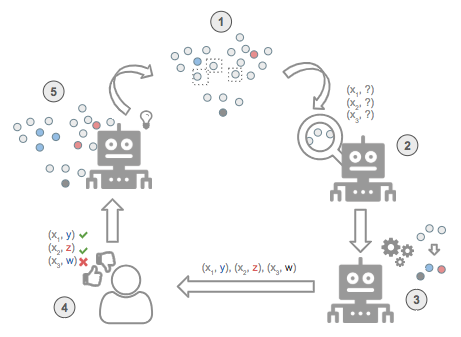
\includegraphics[width=0.9\textwidth]{figures/Framework_Active_Learning_Classico_v2.png}
  \caption{Framework Clássico de Aprendizado Ativo}
  \label{fig:framework_AL_classico}
\end{figure}


O aprendizado ativo costuma ser descrito na literatura em duas grandes etapas: i) cenários e ii) estratégia de seleção e organização das amostras [\cite{settles2014active}]. A etapa de seleção de cenários é a forma pela qual o algoritmo tem acesso aos dados. Existem diversos cenários que podem ser usados mas, independente de qual seja o escolhido, deve-se selecionar qual amostra será enviada para o oráculo através de uma função de utilidade [\cite{olsson2009literature, dasgupta2011two}]. A seguir temos a descrição detalhada dos cenários e estratégias de seleção. 


\section{Cenários do Aprendizado Ativo}
\label{sec:cenarios}

Existem diferentes cenários onde o Aprendizado Ativo poderá fazer a seleção de queries. Dentro desses, os três principais que podem ser considerados na literatura são: (i) membership query synthesis, (ii) stream-based selective sampling e (iii) pool-based sampling [\cite{settles2014active}]. A figura ~\ref{fig:ActiveLearningScenarios} abaixo sintetiza a ideia.


\begin{figure}
  \centering
  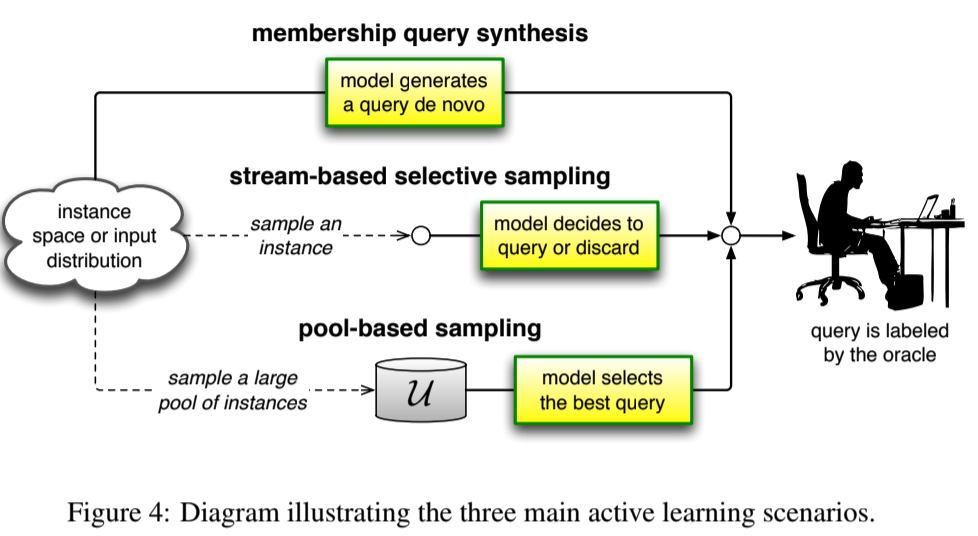
\includegraphics[width=.8\textwidth]{figures/active_learning_scenarios.png}
  \caption{Cenários de Aprendizado Ativo (Settles, 2014)}
  \label{fig:ActiveLearningScenarios}
\end{figure}


\subsection{Membership Query Synthesis}
\label{sec:cenarios_membeship}

Uma das primeiras formas de se pensar na disponibilização dos dados foi atráves do método de membership. Neste cenário, é proposto que o algoritmo crie exemplos sintéticos para serem enviados ao oráculo. Os primeiros trabalhos que utilizaram essa ideia datam de 1980 [\cite{shapiro1981algorithm, shapiro1982algorithmic, shapiro198algorithmic_2}] e há muitas formas de se fazer isso. A única premissa é que o algoritmo possua uma definição dos dados (por exemplo as dimensões da imagem). Para criar novos exemplos podemos, por exemplo, mudar a estrutura de uma imagem ou retirar partes dela.

De uma forma geral o que pretende-se fazer com esse cenário é, na distribuição do espaço de features, criar exemplos representativos. O trabalho de [\cite{baum1992query}] é um bom exemplo pois tentam sintetizar uma amostra através de uma rede neural de 2 camadas. A ideia geral, neste exemplo, é que, dada duas amostras, $x_+$ e $x_-$, das classes positiva e negativa, tenha como objetivo encontrar o melhor hiperplano que as separe. Para isso, sintetiza-se uma amostra m no meio de ambas e pede ao oráculo que nomeie a respectiva classe. Se, por exemplo, a amostra sintética m pertencer a classe $x_+$, sabe-se que o hiperplano deverá estar entre as amostras m e $x_-$. A figura ~\ref{fig:LangBaum_GeometryQueryLearning} representa essa ideia. 

\begin{figure}
  \centering
  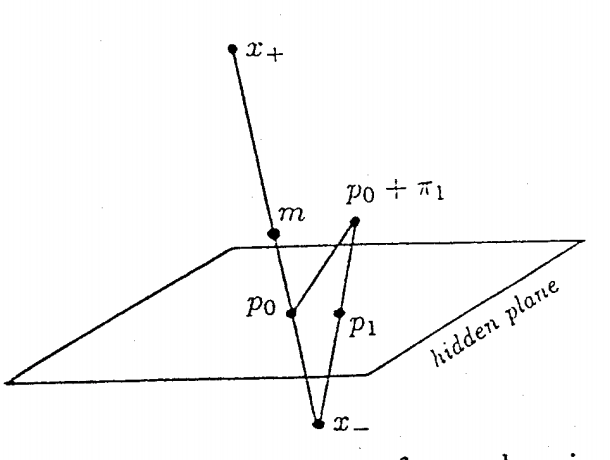
\includegraphics[width=.4\textwidth]{figures/lang_baum_geometry_query_learning.png}
  \caption{A geometria do Aprendizado por Consulta [\cite{baum1992query}]}
  \label{fig:LangBaum_GeometryQueryLearning}
\end{figure}

É importante ressaltar que há desafios nesse sentido quando temos um domínio de alta complexidade, como o caso de imagens de raio-x, por exemplo [\cite{angluin1988queries}]. Mesmo em casos que poderiam ser mais simples encontramos dificuldades. Uma das principais limitações, acontecem quando o oráculo é um humano. Na imagem ~\ref{fig:LangBaum_5vs9Example}, os autores, [\cite{baum1992query}], utilizaram da ideia acima para gerar exemplos sintéticos de imagens de números. O interessante é que, dependendo, de onde os pontos estavam dispostos, algumas imagens não possuíam nenhum significado. Inclusive, o oráculo poderia dar como resposta que determinada amostra era "não reconhecida".

\begin{figure}
  \centering
  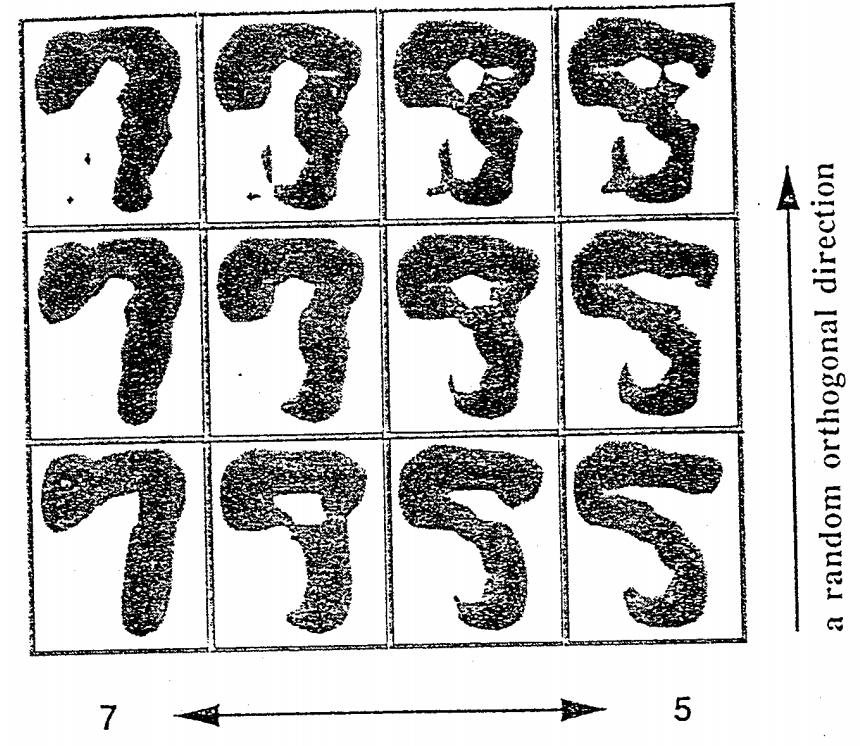
\includegraphics[width=.4\textwidth]{figures/lang_baum_5_vs_9_example.png}
  \caption{Exemplos Sintéticos sem Significado [\cite{baum1992query}]}
  \label{fig:LangBaum_5vs9Example}
\end{figure}

Apesar dessa limitação para oráculos humanos, o trabalho [\cite{king2004functional, king2009automation}] conseguiu utilizar eficientemente essa ideia para quando o oráculo é um robô. Além desse, há um trabalho que utilizou de Genrative Adversarial Networks (GAN) em conjunto com Aprendizado Ativo para criar exemplos [\cite{zhu2017generative}]. O interessante é que eles revisitaram o trabalho de Lang e Baum e conseguiram criar exemplos significativos no caso de dígitos, conforme ilustrado na figura ~\ref{fig:GAN_5_vs_9}. Entretanto, geraram amostras sem significado para fotos de cães e gatos. 

\begin{figure}
  \centering
  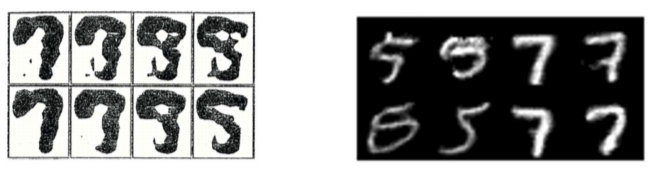
\includegraphics[width=.9\textwidth]{figures/generative_GAN_AL_5_vs_9.png}
  \caption{Esquerda: exemplo de \cite{baum1992query} revisitado e na foto à direita o exemplo gerado pela GAN. [\cite{zhu2017generative}]}
  \label{fig:GAN_5_vs_9}
\end{figure}


Há, ainda, outras iniciativas com esse cenário. No trabalho de [\cite{wang2015active}], por exemplo, utiliza-se o paradigma de criar exemplos sintéticos mas, ao final, utiliza-se exemplos da própria base de dados para serem enviados ao oráculo. Para isso seleciona-se um par de amostras {$x_+$, $x_-$} que estão separadas por um hiperplano e, então, sintetiza-se uma amostra que estará posicionada no meio, adicionada por um pequeno vetor ortogonal. A partir desta amostra sintética, seleciona-se o vizinho mais próximo que será apresentado para o oráculo. O fato de se adicionar um vetor no ponto do meio é para que as amostras sintéticas não fiquem tão concentradas na borda do hiperplano, mas estejam dispersas em torno dele. Além disso, os autores escolheram, a partir da amostra sintética, selecionar o vizinho mais próximo pois ele poderia ser reconhecido por um humano. A figura ~\ref{fig:wang_2015_membership}  mostra essa ideia. O ponto 1, por exemplo, foi criado a partir das amostras $x_+$ e $x_-$. A próxima etapa seria encontrar o vizinho mais próximo de outro par de pontos.

\begin{figure}
  \centering
  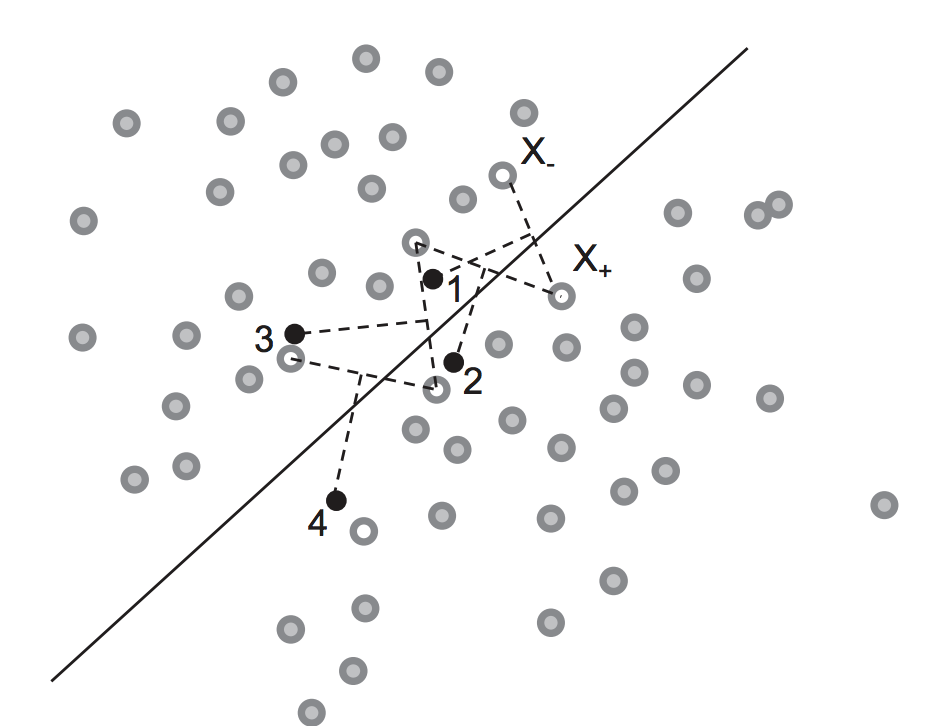
\includegraphics[width=.5\textwidth]{figures/wang_2015_membership.png}
  \caption{Exemplos representativos a partir da posição de amostras sintéticas [\cite{wang2015active}].}
  \label{fig:wang_2015_membership}
\end{figure}


\subsection{Stream-based Selective Sampling}
\label{sec:cenarios_selective_sampling}

Neste cenário permanece a premissa de que obter amostras possui um baixo custo. No entanto, as amostras são sequencialmente disponibilizadas e, através de alguma medida quantitativa, seleciona-se determinada amostra para ser levada ao oráculo ou, então, ser descartada [\cite{settles2014active}]. A figura ~\ref{fig:settles_2014_selective_sampling} mostra o fluxo. 

\begin{figure}
  \centering
  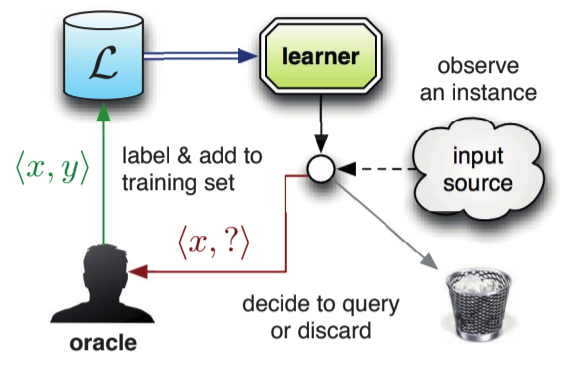
\includegraphics[width=.5\textwidth]{figures/settles_2014_selective_sampling.png}
  \caption{Fluxo do cenário de Selective Sampling [\cite{settles2014active}].}
  \label{fig:settles_2014_selective_sampling}
\end{figure}


Há algumas situações específicas pelas quais é interessante utilizar o cenário sequencial de amostras. A mais comum é quando temos, por exemplo, uma limitação no poder computacional ou de memória. Nesses casos torna-se inviável processar o conjunto de dados sem rotulação de uma única vez. Outro exemplo interessante é quando temos aplicações na web. Nesses casos, também chamado de Online Learning, é interessante que as amostras sejam escolhidas de maneira sequencial. O trabalho de [\cite{chu2011unbiased}], motivado pelos milhões de dados diários do Yahoo, mostra como esse cenário pode ser benéfico. 




\subsection{Pool-based Sampling}
\label{sec:cenarios_pool}

Dos três cenários conhecidos na literatura, o pool-based é o mais utilizado em casos reais, enquantos os anteriores são mais comuns em trabalhos teóricos. Diferentemente do cenário de selective sampling, onde uma das motivações era a falta de recursos, como poder computacional ou memória, aqui escolhemos, de inicio, todo o conjunto de dados. Assume-se, neste caso, que tenhamos um conjunto muito grande de dados sem rótulos e um pequeno conjunto de amostras rotuladas. Também temos que esse conjunto seja estático, embora isso não seja estritamente necessário. A maior diferença entre os dois é que enquanto o primeiro escolhe as amostras sequencialmente e, então, decide, o pool-based analisa todas as amostras e, baseado em uma medida de relevância, seleciona as amostras [\cite{settles2014active}]. A imagem ~\ref{fig:settles_2014_pool}  demostra o fluxo.

\begin{figure}
  \centering
  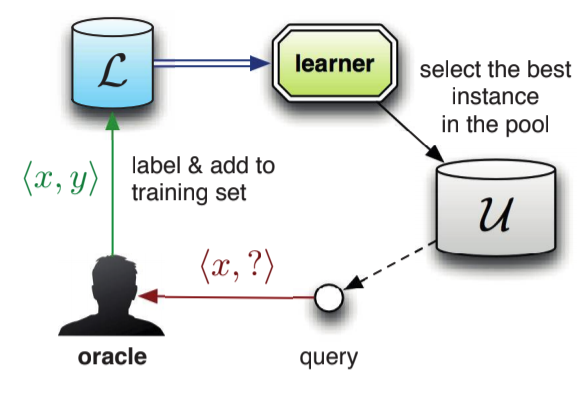
\includegraphics[width=.5\textwidth]{figures/settles_2014_pool.png}
  \caption{Fluxo do cenário de Pool-Based Sampling [\cite{settles2014active}].}
  \label{fig:settles_2014_pool}
\end{figure}

%Existem muitos trabalhos recentes que utilizam esse cenário. Por exemplo: \todo{citar trabalhos}



\section{Estratégia de Seleção e Organização das Amostras}
\label{sec:query_strategy}

Todos os cenários de Aprendizado Ativo discutidos anteriormente envolvem avaliar a relevância das amostras a serem selecionadas. Na literatura, há muitas estratégias formuladas para se fazer isso e, a seguir, temos as principais delas [\cite{settles2012active}]. É importante notar que em todas as estratégias teremos alguma medida quantificável para selecionar as amostras. Por vezes podemos ter estratégias diferentes que utilizam medidas iguais ou similares.




\subsection{Amostras Incertas} %uncertainty sampling 
\label{sec:amostras_incertas}

Amostras Incertas é uma das estratégias mais utilizadas em Aprendizado Ativo. Isso acontece provavelmente por ser muito intuitiva e de fácil implementação [\cite{settles2014active}]. A ideia básica é que precisamos encontrar exemplos que, por terem um alto grau de incerteza, serão os mais relevantes. Ou seja, queremos descartar exemplos nos quais o classificador já possui uma alta confiança de acerto e focar nos exemplos mais incertos.  


\begin{figure}
  \centering
  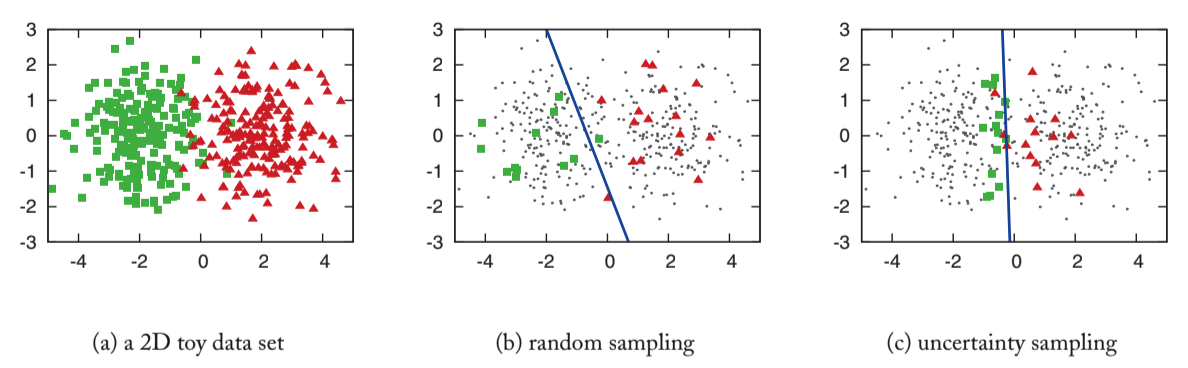
\includegraphics[width=1.0\textwidth]{figures/settles_2014_uncertainty_sampling_example.png}
  \caption{Exemplo de Amostras Incertas [\cite{settles2014active}].}
  \label{fig:settles_2014_uncertainty_example}
\end{figure}

A figura ~\ref{fig:settles_2014_uncertainty_example} exemplifica bem a ideia exposta. Nela temos como classificador uma regressão logística treinada em (b) por 30 amostras aleatórias e em (c) por 30 amostras mais relevantes. É perceptível que, comparando as duas imagens (a) e (b), o classificador obtido através das amostras incertas é o melhor. Isso ocorre porque as amostras mais relevantes estarão, nesse caso, próximas da linha vertical que separa os dois grupos de dados.

Apesar da ideia ser intuitiva precisamos encontrar uma forma de medir a incerteza das amostras. É importante notar que uma interpretação probabilística pode ajudar. Isso porque, quando colocamos nesse escopo, conseguimos generalizar e modelar essa ideia para uma enorme quantidade de casos. Sendo o $x^*_{A}$ a melhor consulta possível utilizando a medida $A$, podemos pontuar as três principais formas de medir a incerteza de uma amostra, que serão expostas abaixo [\cite{settles2014active}].


\textbf{Menos Confiante:} nessa forma estamos interessados nos exemplos nos quais temos menos certeza sobre seu rótulo.
\begin{align*}
\textbf{X}^*_{LC} = &\arg\min_{x} P_{\theta}  (\hat{y}\lvert x)\\
& = \arg\max_{x} 1 - P_{\theta}  (\hat{y}\lvert x),\\
\end{align*}

onde, $\hat{y} = \arg\max_{y} P_{\theta} (y\lvert x)$ e x representa as amostras do dataset, com x $\in$ $\mathbb{R}^n$, e que podem ser classificadas com diferentes classes, y $\in$ \{0, 1, ..., c\}. Assim, para cada x, o $\hat{y}$ é a maior probabilidade que determinada amostra tem de ser rotulada. O que a formula acima faz é olhar a probabilidade condicional na qual, em todos as possíveis amostras, possuirá o menor $\hat{y}$. Desta forma estamos selecionando as amostras mais relevantes para o framework.


Para ilustrar melhor essa ideia, suponha um exemplo onde para cada x $\in$ $\mathbb{R}^n$, temos um $\hat{y}$ de maior probabilidade. Considere um exemplo onde temos duas classes possíveis, y = [0,1]. Uma amostra qualquer $x_q$ terá, portanto, duas probabilidades condicionais para seu $\hat{y}$: P($y_0 \lvert x_q$) e P($y_1 \lvert x_q$). Como o interesse é maximizar a função, escolheremos o $\hat{y}$ de maior probabilidade. A partir disso teremos um conjunto de amostras de X com seus respectivos $\hat{y}$ e escolhemos, entre eles, a amostra mais relevante, isto é, que possui a menor probabilidade. A desvantagem dessa abordagem é que ela considera apenas a informação da melhor predição.  


\textbf{Margem:} similar a medida anterior, a margem tenta resolver a limitação de olhar apenas a melhor predição e utiliza da primeira e segunda maiores probabilidades. 


\begin{align*}
\textbf{X}^*_{M} = &\arg\min_{x}[ P_{\theta} (\hat{y_{1}}\lvert x) - P_{\theta} (\hat{y_{2}}\lvert x)]\\
&\arg\max_{x}[ P_{\theta} (\hat{y_{2}}\lvert x) - P_{\theta} (\hat{y_{1}}\lvert x)]\\
\end{align*}

Intuitivamente, para determinada amostra, caso a margem fique muito alta, significa que o classificador possui uma alta probabilidade em relação à primeira das duas maiores predições possíveis. Ao contrário, caso a margem fique estreita, o classificador não sabe ao certo qual das duas possibilidades determinada classe pertence. Suponha por exemplo que as maiores probabilidades são 0.55 e 0.40, resultando em 0.15. É difícil ter certeza qual das duas são mais relevantes para o framework. Ao contrário, suponha o exemplo onde sejam 0.90 e 0.02, resultando em 0.88. Nesse caso a probabilidade que seja a primeira amostra é muito alta em relação a segunda. Essa abordagem é interessante pois considera informações adicionais para selecionar as amostras. Entretanto, caso tenhamos um número alto de possibilidades, essa abordagem ainda não olha para toda a distribuição possível dos dados.

\textbf{Entropia:} a medida mais geral e comum leva em consideração todas as probabilidades condicionais que uma amostra pode ser classificada. Isto é, tem-se uma probabilidade condicional para cada x, $P(y\lvert x)$, e uma respectiva classe, y$\in$Y. A partir disso calcula-se a entropia H.

\begin{align*}
\textbf{X}^*_{H} = &\arg\max_{x} H_{\theta}  (Y\lvert x)\\
&\arg\max_{x} \sum_{y} P_{\theta}  (y\lvert x) \log_{} P_{\theta}  (y\lvert x),\\
\end{align*}

onde y engloba todas as possíveis classes para cada x. A entropia é máxima quando $P(y\lvert x)$ é uniforme. Dessa forma estamos olhando para todo o conjunto de possibilidades e selecionando as amostras mais incertas.


\begin{figure}
  \centering
  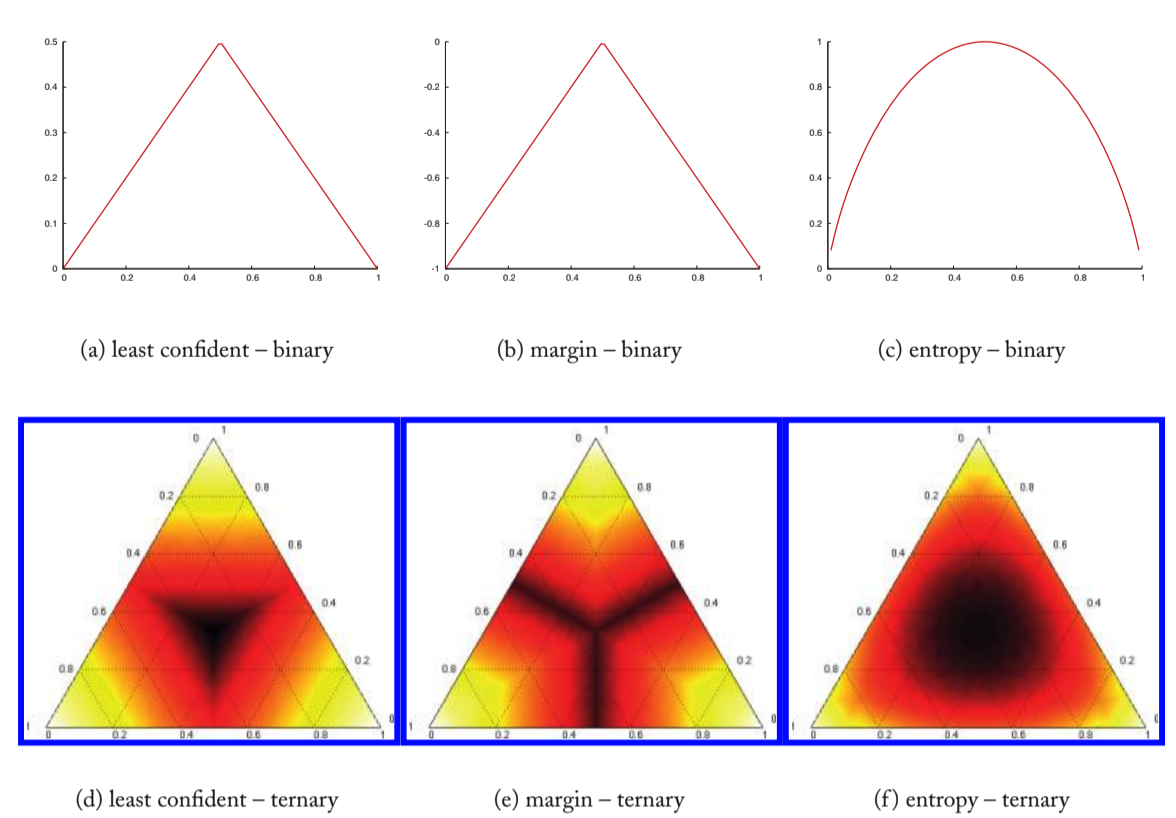
\includegraphics[width=0.8\textwidth]{figures/settles_2014_uncertainty_medidas.png}
  \caption{Comparação entre as três medidas [\cite{settles2014active}].}
  \label{fig:settles_2014_uncertainty_medidas}
\end{figure}



Uma forma de comparar as três medidas pode ser vista na figura ~\ref{fig:settles_2014_uncertainty_medidas}. Nela é possível ver o resultado das funções de relevância em termos da função da probabilidade condicional de determinada classificação, $P(y\lvert x)$. Assim, a parte superior da figura mostra, em um exemplo de classificação binária, que quando a probabilidade da classificação for 0.5, teremos o resultado de maior relevância, pois essa seria a amostra mais incerta. Da mesma forma, na parte inferior, em um exemplo com três possíveis classificações, percebemos a mesma coisa. 


\subsection{Espaço de Hipóteses} 
\label{sec:hypothesis_space}

Uma outra estratégia que pode ser utilizada é procurar amostras dentro do espaço de hipóteses [\cite{mitchell1978version, mitchell1982generalization}]. Nessa estratégia trabalharemos, por exemplo, com mais de um classificador ou com configurações diferentes de um mesmo classificador. Essa ideia foi implementada no trabalho de [\cite{atlas1990training,cohn1994improving}] e pode ser vista na figura ~\ref{fig:cohn_1994_hypothesis_space_example}. Nela temos dois tipos de classificações (0 ou 1) e quatro hipóteses diferentes. As áreas mais escuras, onde há a interseção das diferentes hipóteses, representam a região onde podem haver as amostras mais incertas. 

\begin{figure}
  \centering
  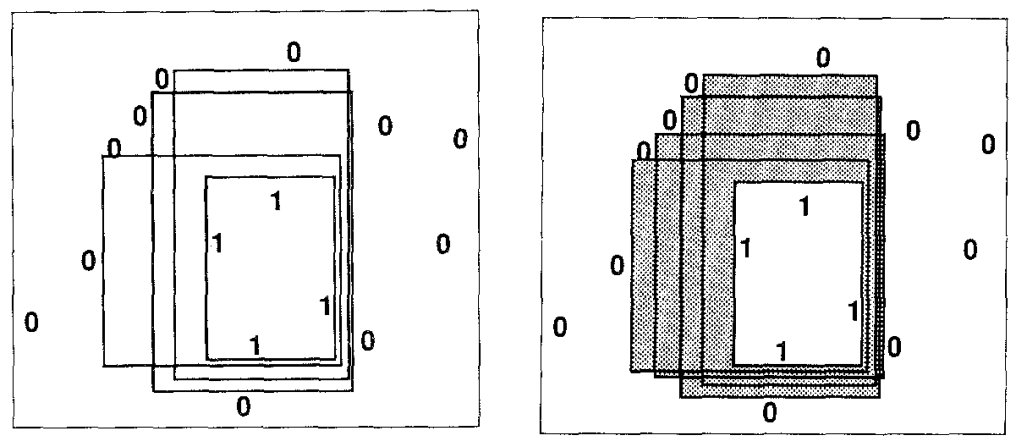
\includegraphics[width=0.7\textwidth]{figures/cohn_1994_hypothesis_space_example.png}
  \caption{Exemplo Espaço de Hipóteses [\cite{cohn1994improving}].}
  \label{fig:cohn_1994_hypothesis_space_example}
\end{figure}

Um outro exemplo mais canônico pode ser visto no trabalho de [\cite{dasgupta2011two}], no qual temos quatro classificadores lineares e a região em rosa representa a área de incerteza. Nessa estratégia uma amostra só iria ser selecionada se estivesse nessa região.

\begin{figure}
  \centering
  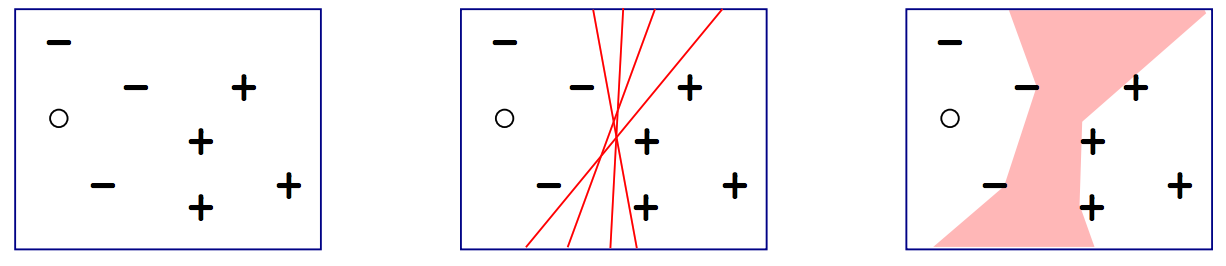
\includegraphics[width=0.9\textwidth]{figures/dasgupta_two_faces_hypothesis_example.png}
  \caption{Exemplo Espaço de Hipóteses [\cite{dasgupta2011two}].}
  \label{fig:dasgupta_two_faces_hypothesis_example}
\end{figure}


A principal forma de procurar amostras dentro do espaço de hipóteses se dá através de consultas por comitês [\cite{seung1992query}]. De uma forma geral, a ideia é que tenhamos um comitê de duas ou mais hipóteses iniciais e, em cada interação onde uma amostra é selecionada, tem-se alguma heurística para mensurar o desacordo entre elas. É importante notar que se o espaço de hipóteses for bem definido e os dados livres de ruído é possível escolher randomicamente um número de hipóteses e usar algum método para estimar o desacordo. Para os casos em que isso não é possível, a literatura apresenta muitas formas de resolver a questão, como uma abordagem bayesiana ou um ensemble de modelos. Não existe uma regra para o número de hipóteses a serem escolhidos. A literatura mostra como comum algo entre cinco a quinze hipóteses, mas pode funcionar bem com duas ou três também [\cite{settles2014active}]. 


Assim como ocorre na estratégia anterior, é necessário que tenhamos como medir a incerteza entre as diversas hipóteses. Existe uma variedade de formas de se fazer isso, mas uma das mais comuns é uma generalização da formula anterior de amostras incertas utilizando a entropia.

\textbf{Entropia por Voto:} a abordagem sugerida por [\cite{dagan1995committee}] considera todas os possíveis rótulos e o número de votos recebidos no comitê. 

\begin{align*}
\textbf{X}^*_{SVE} = - &\arg\max_{x} \sum_{y} P_{C}  (y\lvert x) \log_{} P_{C}  (y\lvert x),\\
\end{align*}

onde y contempla todos as possíveis classes, C é o número de hipóteses e $P_{C}  (y\lvert x) = \frac{1}{|C|}  \sum_{\theta \in C} P_{\theta}  (y\lvert x)$ é a média ou o consenso com maior probabilidade que y está correto, de acordo com o comitê. Novamente a vantagem de utilizar a entropia é que considera-se todas as possíveis classes em todas as possíveis hipóteses, selecionando a amostra de maior relevância.


\subsection{Amostras Incertas vs. Espaço de Hipóteses} 
\label{sec:minimizing_expected}

Uma das limitações das Amostras Incertas está no fato de que, como trabalha-se com uma região específica de dados, é possível que ocorra um processo de aprendizado míope, uma vez que foca-se em uma região particular de dados.  [\cite{settles2014active}]. A parte superior da figura ~\ref{fig:limitations_incertas} ajuda a exemplificar esse problema e a comparação com o espaço de hipóteses. Nela temos (a) o output desejado, (b) alguns dados selecionados de forma randômica, (c) uma rede neural que fez 100 interações de forma randômica, (d) 100 interações utilizando a técnica de amostras incertas e, por último, (e)100 interações utilizando o espaço de hipóteses. É perceptível que o classificador treinado com dados randômicos (c) gerou uma imagem muito distante do output verdadeiro, enquanto o espaço de hipóteses (e) é muito mais próximo dos dois triângulos (a). Além disso, apesar das amostras incertezas (d) lembrarem algo próximo a dois triângulos, continua sendo inferior ao espaço de hipóteses. É interessante notar também a evolução dos classificadores, respectivamente para 20, 40, 60, 80 e 100 interações através da técnica de espaço de hipóteses (fileira do meio da figura) e pelas amostras incertezas (parte inferior da figura).

\begin{figure}
  \centering
  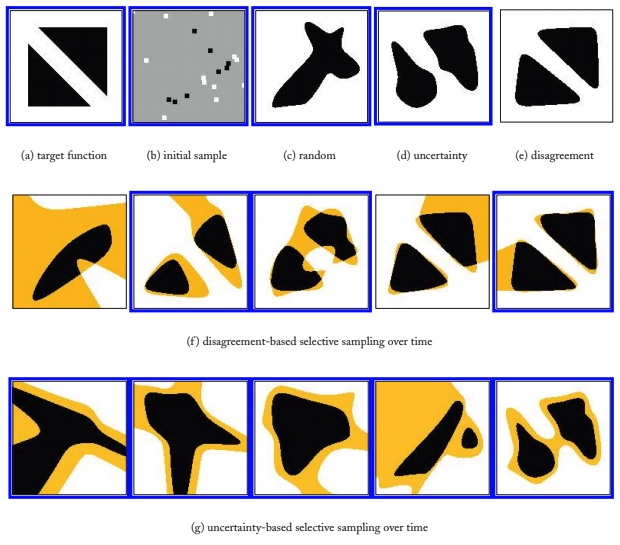
\includegraphics[width=0.7\textwidth]{figures/limitations_incertas.png}
  \caption{Limitações Amostras Incertas [\cite{settles2014active}].}
  \label{fig:limitations_incertas}
\end{figure}

Uma outra limitação, tanto das Amostras Incertas quanto do Espaço de Hipóteses, está no fato de que elas são muito sensíveis a outliers. Isso ocorre porque, nas duas estratégias, as amostras são medidas individualmente [\cite{settles2014active}]. Ou seja, não é levado em consideração a distribuição delas. A figura ~\ref{fig:limitations_outliers} ajuda a sintetizar esse caso. Nela o exemplo A seria o escolhido pois está exatamente na linha de divisão entre as duas classes. Entretanto, por ser um outlier, não é um exemplo realmente relevante. 


\begin{figure}
  \centering
  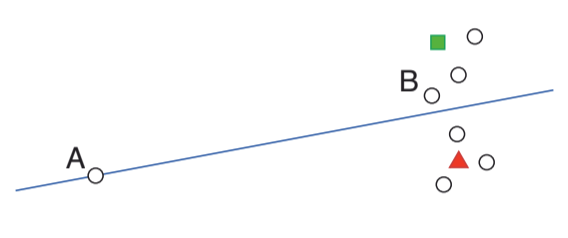
\includegraphics[width=0.5\textwidth]{figures/limitations_outliers.png}
  \caption{Limitações napresença de Outliers [\cite{settles2014active}].}
  \label{fig:limitations_outliers}
\end{figure}

 \subsection{Explorando a Estrutura dos Dados} 
\label{sec:explorando_estrutura_dados }

Uma das maneiras encontradas para resolver a limitação dos outliers é explorar a estrutura dos dados. Uma das formas interessantes de se fazer isso é utilizando a intersecção do Aprendizado Ativo com o Aprendizado Semi-Supervisionado. Podemos, por exemplo, encontrar clusters através de alguma medida de similaridade e utilizar essa informação estrutural. [\cite{saito2014active, dasgupta2011two}]. Selecionamos os centroides e pedimos para o oráculo categorizar corretamente, iniciando, assim, o ciclo do aprendizado ativo. 

Há, porém, alguns problemas na estratégia pois não temos um número óbvio de clusters. Também podemos ter vários níveis de granularidade e, o pior dos casos, os clusters podem não representar as categorias corretas do dataset [\cite{dasgupta2011two, settles2014active}].  A figura ~\ref{fig:toy_example_clustering} exemplifica essa ideia. A imagem (a) mostra uma distribuição de dados de um espaço de features. Como não temos a informação a respeito das verdadeiras classes desses dados, se aplicarmos um algoritmo não supervisionado para encontrar possíveis padrões e clusters, pode ser difícil saber quantos clusters realmente existem. Algumas possibilidades estão nas figuras b-e, mas isso não significa que representam as classes corretas desse conjunto de dados. 


\begin{figure}
  \centering
  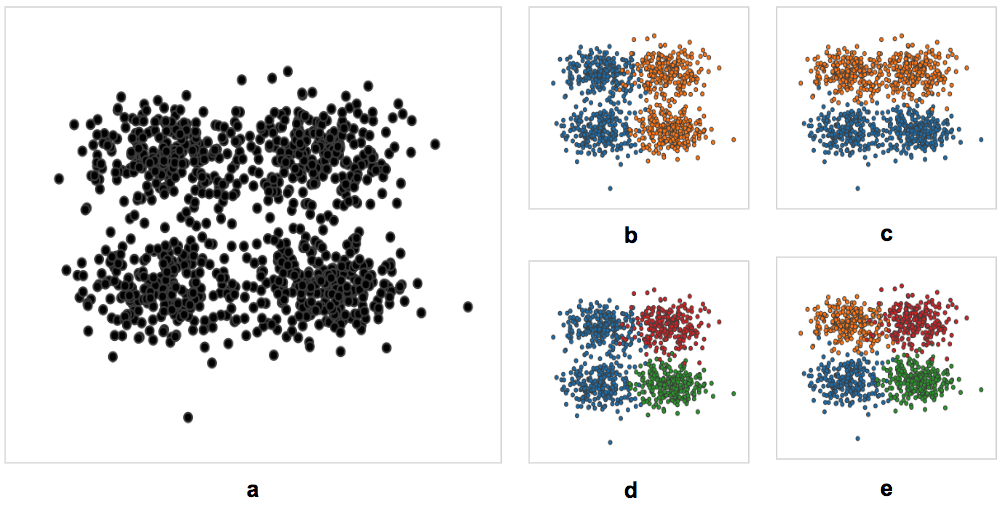
\includegraphics[width=0.9\textwidth]{figures/toy_example_clustering.png}
  \caption{Exemplo de Clustering.}
  \label{fig:toy_example_clustering}
\end{figure}


\section{Aprendizado Ativo com Participação Ativa do Usuário}
\label{sec:aprendizado_ativo_variacoes}

O aprendizado ativo tem como principal objetivo diminuir o esforço gasto na rotulação de amostras e ao mesmo tempo obter um bom classificador. Há outras técnicas que são correlatas a essa ideia, como o aprendizado semi-supervisionado [\cite{zhu2006semi}], que utiliza da própria estrutura dos dados para re-treinar o classificador. Outra técnica interessante é o transfer learning [\cite{rodrigues2018evaluation}], que tem como objetivo passar um conhecimento prévio de um problema já resolvido para algum outro similar. Além desses que foram citados podem existir diversas variações. A diferença básica é que no aprendizado ativo temos a interação de um oráculo, sendo na maioria das vezes um humano. 


Apesar dessa ideia ser muito interessante, principalmente quando temos um domínio que requer profissionais extremamente especializados para categorizar as amostras, o oráculo no framework clássico ainda é utilizado de forma muito limitada [\cite{seifert2010user}]. Nele o papel do oráculo se restringe em aceitar/corrigir as classes dadas pelo classificador. Trabalhos mais recentes vem buscando dar ao oráculo outros papéis. Na realidade, existe um grande interesse em como incorporar mais conhecimento humano dentro dessa estrutura [\cite{settles2014active}]. 

O trabalho de [\cite{castro2009human}] foi um dos primeiros a tentar relacionar, de forma quantitativa, o aprendizado ativo com a ciência cognitiva. Nesse caso o problema era conseguir identificar duas classes de ovos alienígenas que se diferenciavam pela forma. O estudo foi feito com 33 participantes através de três testes: i) aprendizado humano-ativo, ii) aprendizado computador-ativo e iii) randômico. Para cada um dos testes também foi adicionado ruído nos dados. O estudo demonstrou que o aprendizado ativo, tanto com os humanos participando da seleção e correção das classes quanto do aprendizado ativo clássico, é melhor que a forma randômica. Além disso, o aprendizado ativo, com pouco ruído nos dados, é apenas um pouco inferior ao clássico mas, a medida que dados ruidosos foram adicionados, a acurácia diminuiu, conforme mostra a figura ~\ref{fig:human_active_learning_graph}. Um outro estudo parecido feito por [\cite{markant2014better}] mostrou que, para determinados casos, o resultado é semelhante.

\begin{figure}
  \centering
  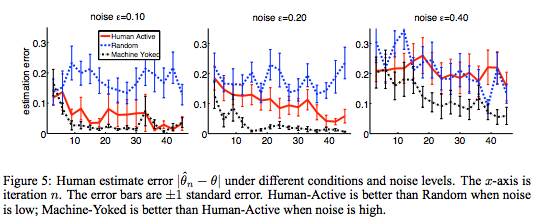
\includegraphics[width=0.9\textwidth]{figures/human_active_learning_graph.png}
  \caption{Exemplo do Estudo feito por Castro et all.}
  \label{fig:human_active_learning_graph}
\end{figure}


%% falar do Castro que eeles querem implementar em casos reais!!!

Um segundo trabalho importante de 2010 foi o de [\cite{seifert2010user}] que também buscou dar ao usuário um papel mais ativo em relação a escolha de amostras. Na pesquisa foi sugerido uma forma de visualizar o espaço de característica dos dados, conforme a o quadro esquerdo da figura ~\ref{fig:seifert_example}. As classes foram dispostas de forma igual em torno do perímetro do circulo. As regiões mais distantes do centro eram consideradas mais certas de serem classificadas com determinado rótulo. Como não foi possível fazer testes com humanos no dataset final, foi feito um experimento anterior com usuários para identificar padrões nos quais os usuários selecionavam amostras. A partir disso foi proposto dois modelos de simulação: i) modelo gaussiano e ii) modelo por convex-hull, conforme o quadro do meio e da direita da figura ~\ref{fig:seifert_example}. Ambos modelos tem como premissa que o usuário seleciona as amostras mais incertas. O primeiro estima que elas estejam no meio, pois é a região de mais incerteza. A diferença para o segundo é que ele também leva em consideração a distribuição dos dados. Os resultados mostraram que um papel ativo do usuário foi superior que o aprendizado ativo clássico para todos os casos e que nunca foi inferior às amostras randômicas, apesar de ter apresentado resultados bem próximos. Um outro ponto interessante da conclusão do estudo é que isso pode variar dependendo da base de dados e do classificador utilizado.

\begin{figure}
  \centering
  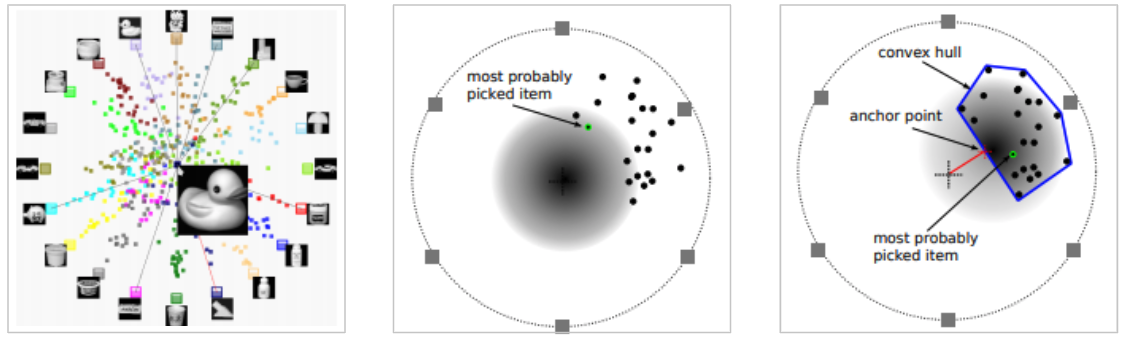
\includegraphics[width=1.0\textwidth]{figures/seifert_example.png}
  \caption{Exemplo do Estudo feito por Seifert e Granitzer.}
  \label{fig:seifert_example}
\end{figure}

O interesse em unir o conhecimento humano, incorporando-o no loop de aprendizado, continua em aberto [\cite{calma2016active}], sendo apoiado por pesquisas da área da psicologia [\cite{sim2015children}]. Um estudo recente [\cite{kottke2018other}] teve como objetivo fazer um experimento com 77 estudantes divididos em 14 grupos, dos quais nenhum deles tinha conhecimentos sobre respeito Aprendizado Computacional. O estudo comparou a acurácia dos grupos em relação à abordagem clássica do aprendizado ativo, assim como a seleção aleatória das amostras. Os resultados mostraram que, no geral, os grupos não tiveram resultados superiores em relação ao framework clássico ou em relação ao framework com amostras randômicas. Apesar disso, quando olhamos para os 5 melhores grupos, tivemos uma acurácia superior. Isso não foi determinado pelo estudo mas talvez os melhores grupos possam ser comparados com usuários experts. 

Além dos estudos abordados acima há outros dois que merecem ser mencionados, os quais analisam a interação de ferramentas visuais no processo de aprendizado ativo. Inclusive há indícios que ambas áreas estão se aproximando [\cite{sacha2016human}]. O primeiro é o trabalho do MapView [\cite{weigl2016mapview}] que propôs uma ferramenta gráfica através da redução de dimensionalidade do espaço de características para um espaço 2D. O estudo não fez comparações com a abordagem clássica de aprendizado ativo ou de amostras randômicas. Na realidade o trabalho propôs essa ferramenta e demonstrou duas principais contribuições para os usuários: i) encontrar possíveis insights em um espaço de features 2D, projetado a partir de um espaço de alta dimensionalidade e ii) através de uma abordagem visual, os usuários puderam ter um melhor entendimento do classificador. 

Um outro trabalho interessante foi o [\cite{bernard2018comparing}] no qual foi feito um estudo experimental comparando o aprendizado ativo e interações visuais. O objetivo foi descobrir se o aprendizado ativo, com uma participação ativa do usuário através de ferramentas visuais, possuía uma melhor acurácia. Além disso, buscou entender se o aprendizado ativo poderia aproveitar dessas técnicas, onde foi proposto um framework de Aprendizado Interativo Visual para rotular amostras. 

\begin{figure}
  \centering
  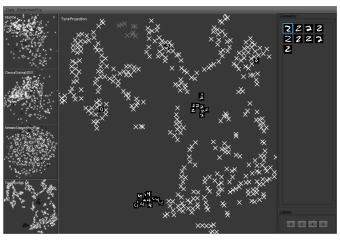
\includegraphics[width=0.8\textwidth]{figures/visual_comparing.png}
  \caption{Exemplo Ferramenta de Aprendizado Visual Interativo.}
  \label{fig:visual_comparing}
\end{figure}


O experimento foi composto por 16 pessoas, que possuíam conhecimentos prévio de análise de dados. Nele foi criado uma ferramenta visual que testou tanto a abordagem com o usuário ativo, quanto com o framework clássico. Para isso, utilizaram de algoritmos de redução de dimensionalidade e o usuário poderia escolher quais amostras ele gostaria de rotular. No framework clássico foi utilizado medidas para estimar as amostras relevantes, como foi comentado no inicio deste capítulo. A figura ~\ref{fig:visual_comparing} mostra a imagem da ferramenta visual. Os quatro pequenos quadros à esquerda representam diferentes algoritmos de redução de dimensionalidade. O usuário escolhe o de sua preferência e inicia o ciclo de escolha das amostras e rotulação. Os resultados mostraram que colocar o humano como centro do framework, com o apoio de ferramentas visuais, conseguiu competir com os modelos clássicos de aprendizado ativo. 








%  O interesse em unir o conhecimento humano, incorporando-o no loop de aprendizado, continua em aberto [\cite{calma2016active}]. Inclusive, há uma linha de pesquisa interessante que pretende fazer isso com o apoio de análises visuais, como a utilização de grafos e projeções em 2D [\cite{yang2018visually, bernard2018comparing, weigl2016mapview}]. Por exenplo, um estudo recente [\cite{kottke2018other}] teve como objetivo mudar a posição do humano de ser um especialista em categorizar amostras para ser também um especialista em selecionar. No estudo foi possível demonstrar resultados positivos, onde o aprendizado computacional pôde se beneficiar com a interação humana. 

%% comentar aqui o rtablaho do settles com NLP

%% falar quer e exclusivamente nos casos onde termos a necessidade de um especialista. Lembrar do trabalho do Baum que nao deu certo (exemplos sinteticos que nao faizam nenhum sentudo!)